\documentclass[a4paper]{article}
\usepackage[T1]{fontenc}
\usepackage[utf8]{inputenc}
\usepackage[italian]{babel}
\usepackage{url}
\usepackage{graphicx}
% == Pacchetti utilizzati per la costruzione della tabella e per l'immagine di copertina ==
\usepackage{booktabs}
\usepackage{ctable}
% == Pacchetto per utilizzare il simbolo dell'euro € == %
\usepackage{eurosym}
% == Pacchetti per l'indice interattivo == %
\usepackage{color}
\usepackage{hyperref}
\hypersetup {
	pdftitle = {Progetto di Ingegneria del Software},
	pdfauthor = {Enrico Pasquali, Alessio Zampieri},
	pdfsubject = {Prototipo di un'applicazione per la gestione di un magazzino},
	pdfkeywords = {.},
	colorlinks = true,
	linkcolor = cyan,
	linktocpage = true,
	pageanchor = true
}
% = Pacchetto per effettuare larghe porzioni di commenti attraverso \begin{comment} \end{comment}


\def\changemargin#1#2{\list{}{\rightmargin#2\leftmargin#1}\item[]}
\let\endchangemargin=\endlist 
\begin{document}
\author{Enrico Pasquali \and Alessio Zampieri}

% =============== PRIMA PAGINA ============================

	\begin{titlepage}
	\begin{center}
		
		{ \huge \bfseries Progetto di Ingegneria del Software \ }
		\rule{11cm}{.4pt} 
		\\ [0.3cm]
		{\large Prototipo di un'applicazione per la gestione di un magazzino.}
		\\ [1cm]
		{ \large A cura di \\  {Enrico Pasquali, Alessio Zampieri} }

    %\vfill
	\end{center}
	\end{titlepage}

% ==================== INDICE =================================	
	\tableofcontents
	\newpage
% ====================== SPECIFICHE ===========================

	\section{Specifiche}
	Si vuole progettare un sistema informatico per gestire il magazzino di una catena di negozi di articoli sportivi.
	
	Il negozio vende articoli di diversa tipologia, raggruppati per sport. Per ogni tipo articolo si registra: un nome univoco, una descrizione, lo sport, e i materiali utilizzati per produrlo. 
	
	Il sistema registra tutti gli articoli in magazzino	memorizzando per ogni articolo: il tipo di articolo, un codice univoco, il prezzo e la data di produzione.
	
	Gli articoli in magazzino vengono gestiti dal sistema che registra per ogni ingresso in magazzino: un codice interno univoco, la data e tutti articoli entrati e le loro posizioni in magazzino. 
	
	Per ogni uscita il sistema registra: la data e il numero di bolla (univoco), tutti gli articoli usciti, il negozio che li ha ordinati e lo spedizioniere che li ritira. 
	
	Per ogni negozio della catena il sistema registra: il codice fiscale, il nome, l’indirizzo e la città.
	
	Il sistema memorizza inoltre gli ordini dei negozi registrando: il negozio che ha effettuato l’ordine, un codice ordine univoco, la data dell’ordine, i tipi di articolo ordinati e per ogni tipo di articolo la quantità ordinata e il prezzo totale.
	
	Quando un ordine viene evaso si registra un’uscita dal magazzino che viene collegata all’ordine al quale si riferisce. Si suppone che per ogni ordine evaso si abbia una sola uscita dal magazzino.
	
	Per ogni tipo di articolo il sistema memorizza esplicitamente alla fine di ogni mese dell’anno la quantità di articoli ricevuti in magazzino e la quantità di articoli usciti.
	
	Il sistema deve permettere ai magazzinieri di inserire le informazioni relative ai movimenti di ingresso e uscita dal magazzino. I magazzinieri, inoltre, possono spostare un articolo da una posizione ad un’altra del magazzino, al fine
	di ottimizzare l’occupazione del magazzino.
	
	La segreteria amministrativa della catena di negozi è responsabil dell’inserimento dei tipi di articolo. Essa può accedere al sistema e visualizzare i movimenti di magazzino rispetto agli ordini dei vari negozi. 
	Tutti gli utenti sono opportunamente autenticati dal sistema, prima che possano accedere alle funzionalità specifiche.
	
	I responsabili dei negozi possono accedere al sistema per effettuare gli ordini e per avere un riassunto degli ordini passati.
	
% ========================= INTRODUZIONE ==============================

	\section{Introduzione}
	Si vuole progettare una base di dati per gestire le informazioni relative
	alla gestione di un magazzino di una catena di negozi di articoli sportivi.
	Gli attori principali del sistema sono:
	\begin{itemize}
		\item La segreteria amministrativa
		\item I responsabili di ciascun negozio della catena
		\item I magazzinieri
	\end{itemize}
	
	Il seguente documento parte quindi da una descrizione ad un alto livello d'astrazione dei concetti fondamentali del sistema, attraverso la presentazione
	di use case e sequence diagram, per poi entrare nel dettaglio con lo
	schema delle classi e la descrizione dei principali pattern usati.
	Verrà anche poi presentato lo schema ER (entità-relazione) e lo schema fisico
	della base di dati creata per la gestione del sistema.
	L'applicazione prevede l'autenticazione in modo elementare di tutti gli utenti che interagiscono con il sistema.
	Seguiranno infine alcuni esempi di utilizzo dell'applicazione.


	\section{Requisiti utente}
	Vengono evidenziati coloro che sono coinvolti nel progetto e nel successivo utilizzo del prototipo. \\
	\textbf{STAKEHOLDERS}: Segreteria amministrativa, magazzinieri, responsabili dei negozi, progettisti del sistema.

	\subsection{Usecase Diagram}
	Sono presentati di seguito il diagramma dei casi d'uso e le relative schede.
	\\ [2cm]
	\includegraphics[width=1\textwidth, height=0.5\textheight]{Usecase}
	
	\newpage
	
	\subsubsection{Personale}
	\begin{center}
		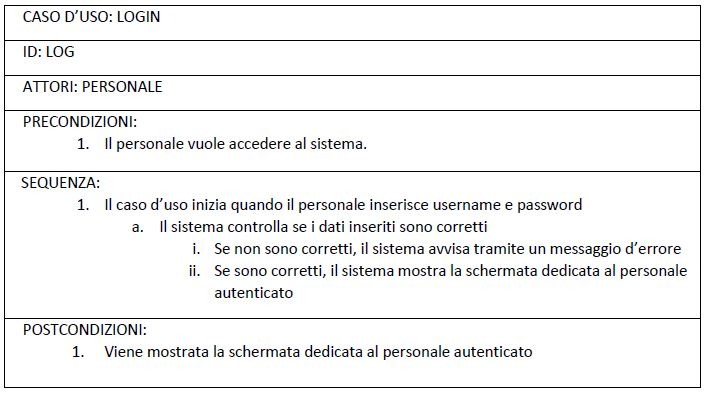
\includegraphics [scale=0.5] {login}
	\end{center}
	
	\subsubsection{Segreteria amministrativa}
	\begin{center}
		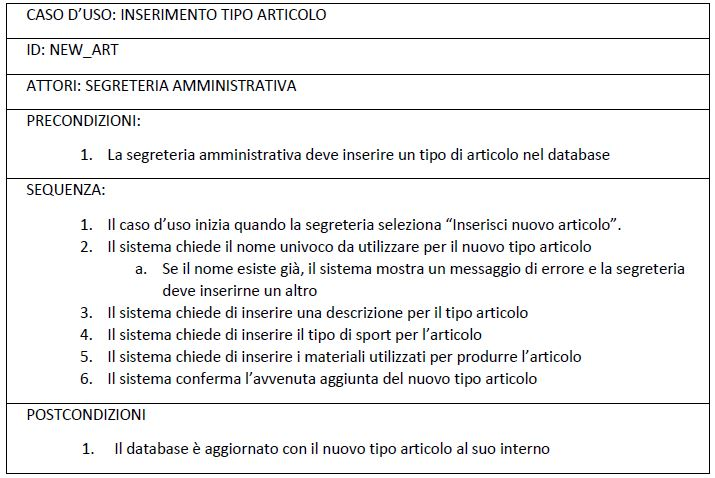
\includegraphics [scale=0.5] {new_article}
	\end{center}
	\begin{center}
		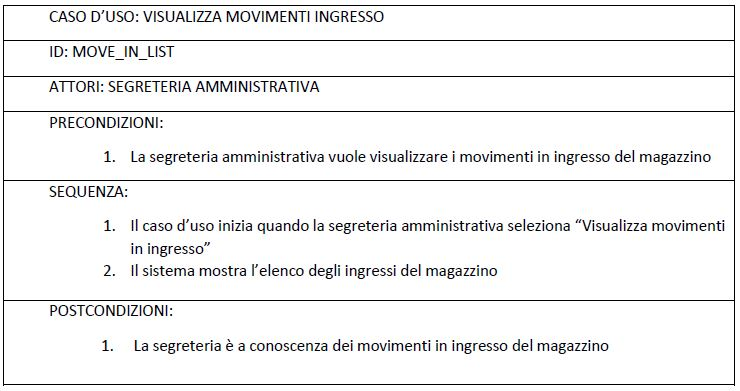
\includegraphics [scale=0.5] {move_in_list}
	\end{center}
	\begin{center}
		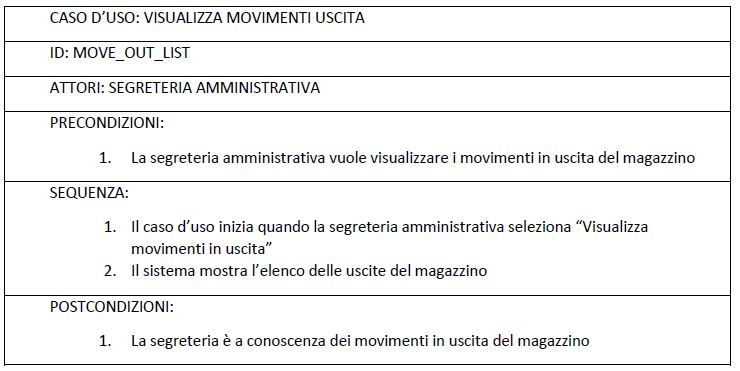
\includegraphics [scale=0.5] {move_out_list}
	\end{center}
	
	\subsubsection{Responsabile negozio}
	\begin{center}
		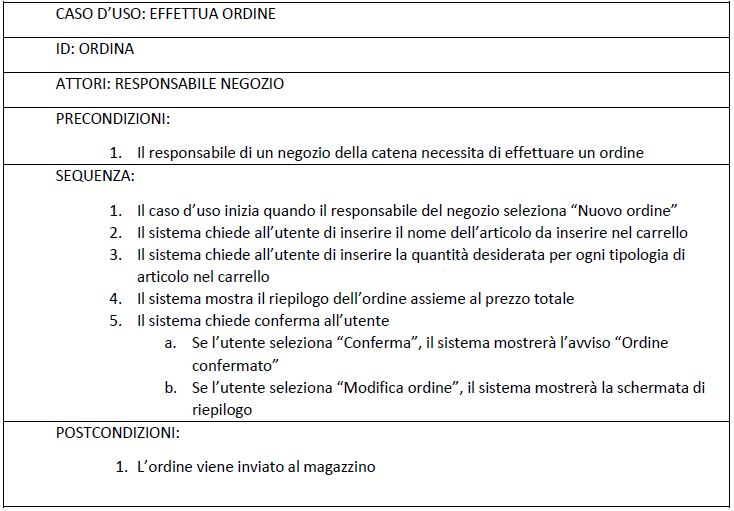
\includegraphics [scale=0.5] {new_order}\\
	\end{center}
		\begin{center}
		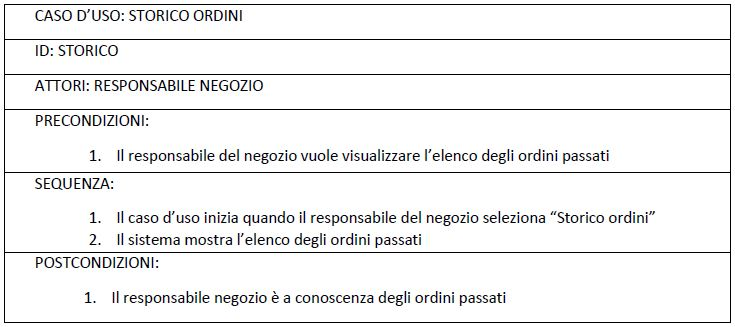
\includegraphics [scale=0.5] {orders_list}\\
	\end{center}

	\subsubsection{Magazzinieri}
	\begin{center}
		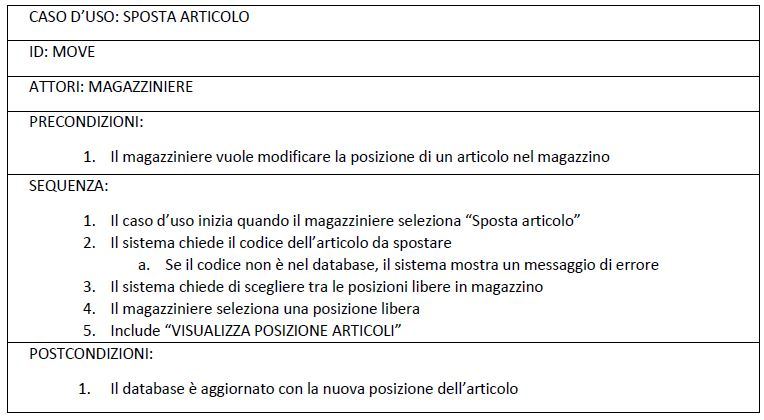
\includegraphics [scale=0.5] {move}\\
	\end{center}
		\begin{center}
		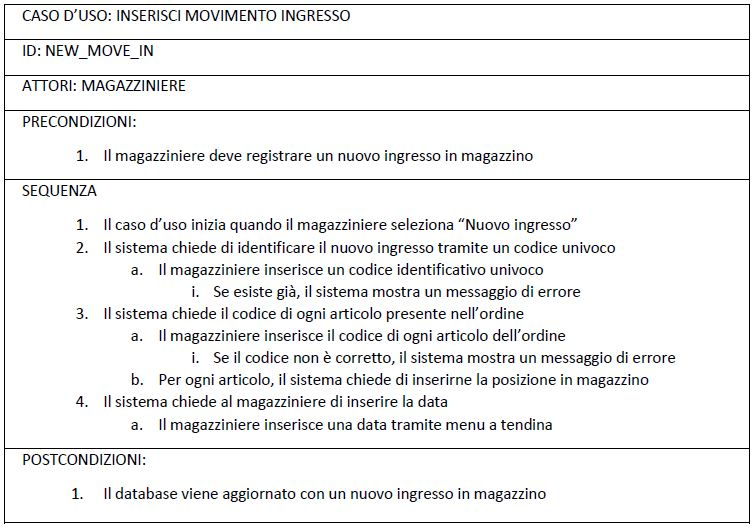
\includegraphics [scale=0.5] {new_move_in}\\
	\end{center}
	\begin{center}
	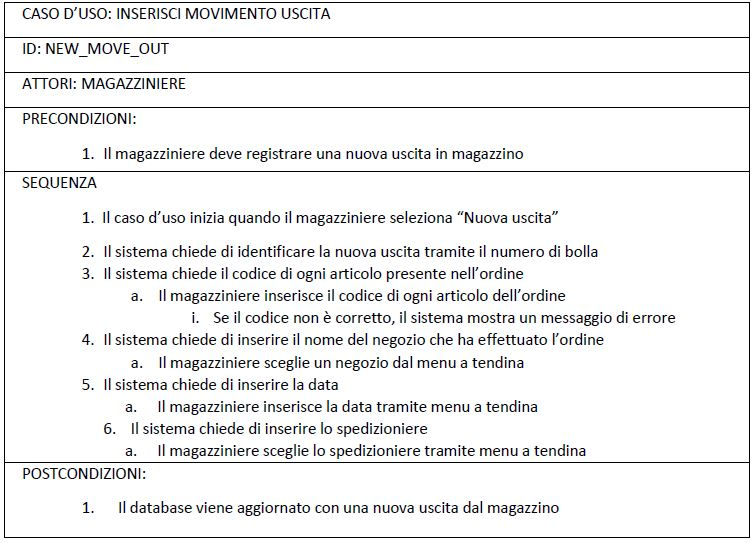
\includegraphics [scale=0.5] {new_move_out}\\
	\end{center}
	
\subsection{Sequence diagram}
I \textit{sequence diagram} dettagliano la sequenza temporale degli eventi che non è possibile rappresentare con gli \textit{use case}.
\\ [0.5cm]

\newpage

\section{Requisiti di sistema}
\subsection{Class Diagram} %\label{cap:4}
Presentati di seguito i \textit{class diagram} sviluppati per il software.\\
In un primo momento, viene visualizzata la struttura generale dove sono evidenziate le relazioni presenti tra le classi. Successivamente si entrer\`a nel dettaglio di ciascuna.\\
Il progetto \`e suddiviso in tre package:
\begin{itemize}
	\item \textbf{controller}, il quale contiene le classi relative al controllo dei dati.
	\item \textbf{model}, il quale contiene le classi per la gestione e recupero dati interfacciandosi con la base di dati.
	\item \textbf{view}, il quale implementa la parte di visualizzazione grafica.
\end{itemize}
I tre package comunicano quindi seguendo il pattern del \textit{Model-View-Controller} (\textbf{MVC}). \\
In figura è mostrata la struttura generale dove: il controller risulta essere in relazione con il model, ricevendo gli eventi dalla view e coordinando le operazioni necessarie.\\[0.5cm]

\subsubsection{Controller}
Ogni attore è quindi gestito nelle sue funzionalit\`a da un Controller distinto. \\ 

\newpage

\subsubsection{Model}
L'implementazione del \textit{Model} invece risulta abbastanza semplice, in quanto la parte importante di gestione e memorizzazione dei dati è concentrata nella \textit{Base di Dati}.\\
Ogni classe esegue le query a cui fa riferimento per poi incapsulare i dati letti e passarli al controller, view e model corrispondente in modo più agevole.\\


\newpage

\subsubsection{View}
Il package \textit{View} contiene le classi che si occupano della realizzazione dell'interfaccia grafica.

\newpage

\subsection{Sequence diagram delle classi}
Qui i \textit{Sequence Diagram} che descrivono a pi\`u basso livello il comportamento delle classi.
\subsubsection{Segreteria amministrativa}
%\newpage
\subsubsection{Responsabile negozio}

\subsubsection{Magazziniere}
 
\newpage

\section{Modelli di sistema}
\subsection{Activity diagram}
Qui i modelli di sistema, ovvero, gli \textit{activity diagram}.

\subsubsection{Segreteria amministrativa}  
\begin{center}
	
	\begin{changemargin}{-1.5cm}{-0.5cm} 
		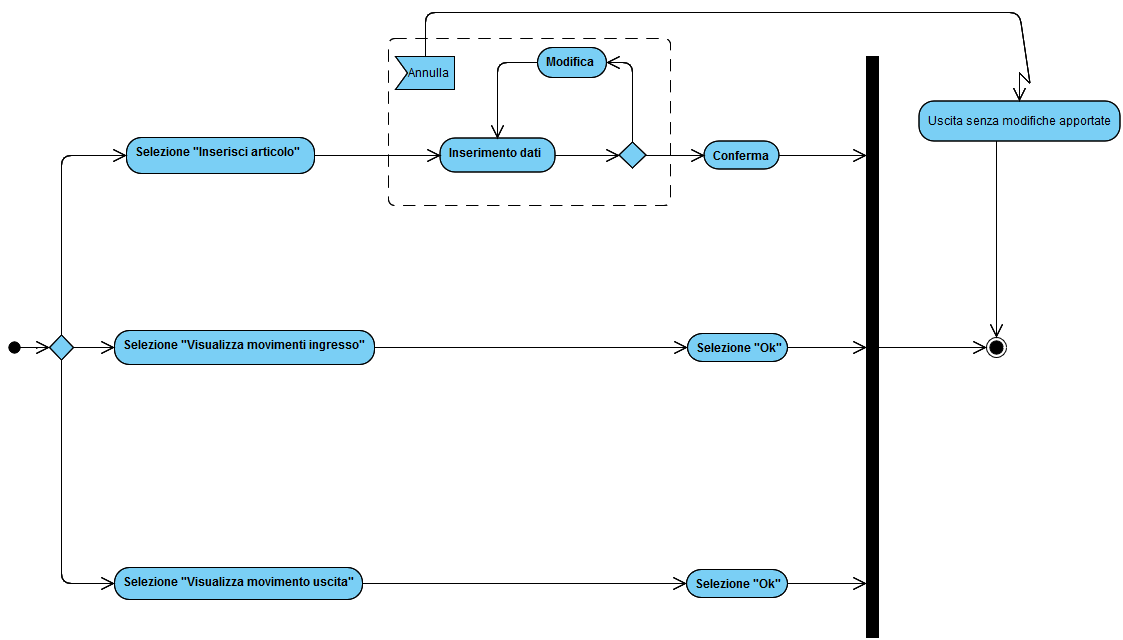
\includegraphics [scale=0.5] {ActivityDiagram_SegreteriaAmministrativa}
	\end{changemargin} 
	
	
\end{center}

\subsubsection{Responsabile negozio}
\begin{center}
\begin{changemargin}{-1.5cm}{-0.5cm} 
	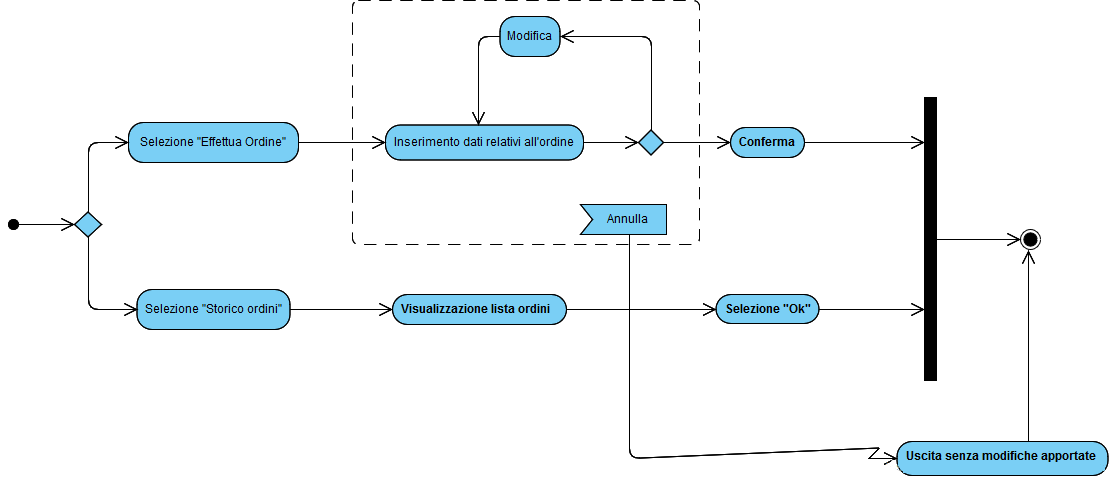
\includegraphics [scale=0.5] {ActivityDiagram_ResponsabileNegozio}
\end{changemargin} 
\end{center}

\subsubsection{Magazziniere}
\begin{center}
	\begin{changemargin}{-1.5cm}{-0.5cm} 
		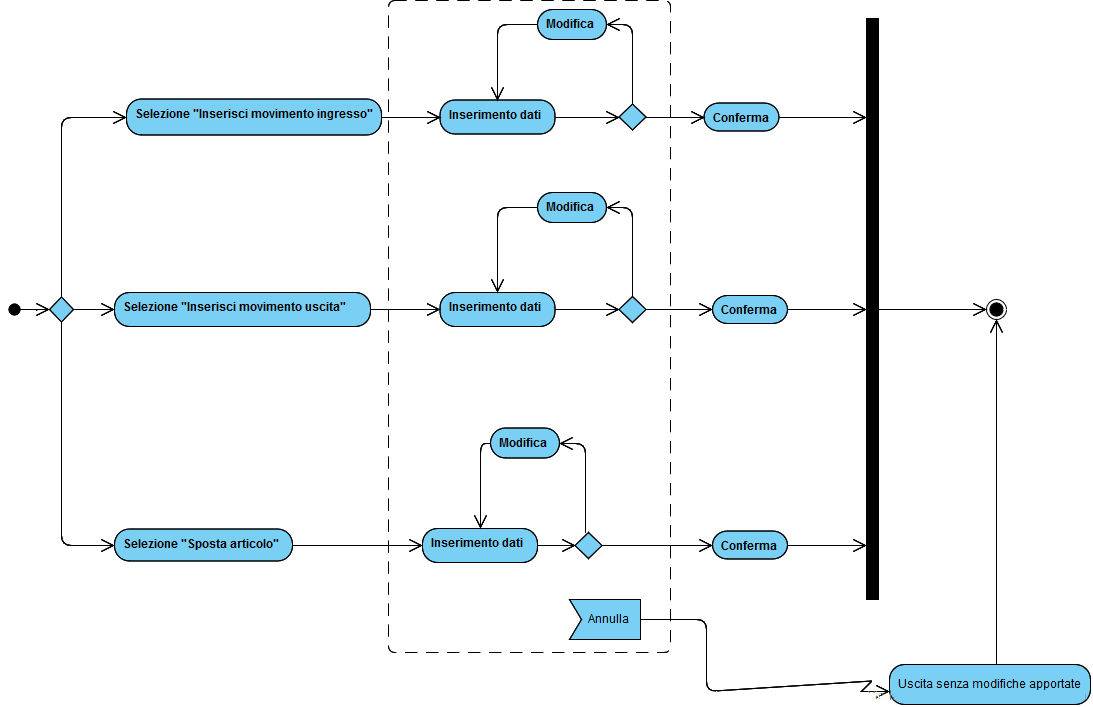
\includegraphics [scale=0.5]  {ActivityDiagram_Magazziniere}
	\end{changemargin} 
\end{center}

\section{Progettazione e sviluppo}
\subsection{I Pattern usati}

\section{Struttura del database}

\textsc{Schema Concettuale}\\
\textsc{Schema Relazionale}\\

I vincoli d'integrit\`a sono: ($DA MODIFICARE$)

	Locale.proprietario $\rightarrow$ Personale.username\\
	Comande.cameriera $\rightarrow$ Personale.username \\
	Comande.tavolo $\rightarrow$ Tavoli.numTavolo \\
	Comande.piatto $\rightarrow$ Listino.piatto\\
	Ricette.piatto $\rightarrow$ Listino.piatto\\
	Ricette.ingrediente $\rightarrow$ magazzino.nomeIngrediente\\


\section{Testing}
\end{document}

